\section{Related Work}
\subsection{Real-time System}
\begin{frame}
  \frametitle{Related Work --- Real-time Systems and EDF}
  Real-time system (RTS) is a different scheme of operating system
  design focused on serving real-time applications.
  \begin{itemize}
    \item Mission oriented.
    \item Jobs are provided with {\emph{hard}} deadlines that cannot be violated.
    \item If the system cannot guarantee to finish a submitted job
      before its deadline, it rejects it.
  \end{itemize}

  Earliest Deadline First algorithm was proved to be an optimal
  scheduling algorithm on preemptive uniprocessors
  \footnote[frame]{\tiny\fullcite{cite:pinedo2012scheduling}}.
  \begin{itemize}
    \item By optimal we mean: If a set of jobs can be scheduled in a way that all the jobs
      can finish before deadline, EDF is able to schedule them.
    \item Takes only deadline into consideration.
  \end{itemize}
\end{frame}
\subsection{Parallel Real-time Job}
\begin{frame}
  \frametitle{Related Work --- Parallel Real-time Job (PRJ) Scheduling}
  PRJs are jobs in parallel real-time systems, where jobs can be run in
  parallel.  Different frameworks and algorithms are proposed for
  different constraints.
  \begin{itemize}
    \item Reliability-Driven method by Qin et al.
      \footnote[frame]{\tiny\fullcite{cite:qin-reliability-driven}}
    \item He et al. viewed it as hybrid of periodic and aperiodic jobs
      and proposed a method by modeling spare capabilities
      \footnote[frame]{\tiny\fullcite{cite:he-spare-capabilities}}
    \item TAPADS by Xie et al. with deadline and security constraints.
      \footnote[frame]{\tiny\fullcite{cite:roystonea}}
  \end{itemize}
\end{frame}
\subsection{SLA Jobs}
\begin{frame}
  \frametitle{Related Work --- Scheduling with SLAs}
  User utility based:
  \begin{itemize}
    \item Libra --- computational economy driven scheduling
      \footnote[frame]{\tiny\fullcite{cite:libra}}
    \item Yeo et al. proposed a framework with linear penalty model on
      user utility.
      \footnote[frame]{\tiny\fullcite{cite:yeo-SLA-penalty}}
  \end{itemize}
  Grid computing
  \begin{itemize}
    \item He et al. proposed a two level optimization --- MUSCLE, a
      multi-cluster level scheduler, and TITAN, a single-cluster level
      workload manager.
      \footnote[frame]{\tiny\fullcite{cite:he-muscle-titan}}
  \end{itemize}
\end{frame}
\subsection{JPPF}
\begin{frame}
  \frametitle{Related Work --- JPPF}
  \begin{columns}
    \begin{column}{.6\textwidth}
      \begin{itemize}
        \item A popular open-source cluster management framework.
        \item Easy to deploy.
        \item Provides an easy to use GUI management tool.
        \item Abundant APIs for customization
          \begin{itemize}
            \item But still hard to achieve node-aware scheduling.
          \end{itemize}
      \end{itemize}
    \end{column}
    \begin{column}{.4\textwidth}
      \resizebox{\linewidth}{!}{
        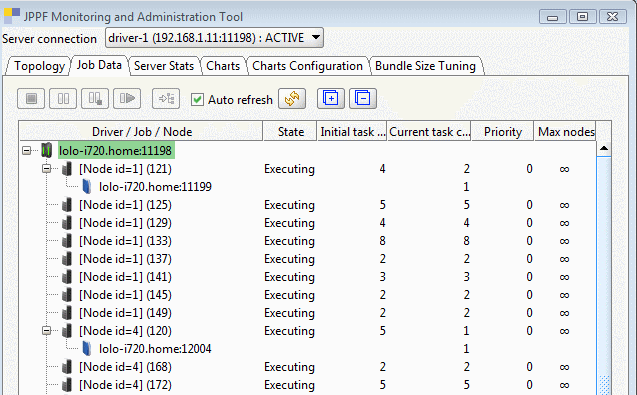
\includegraphics{figures/jppf.png}
      }
      \footnote[frame]{\tiny Picture is from the official site
      http://www.jppf.org}
    \end{column}
  \end{columns}
\end{frame}
